\begin{tikzpicture}
\draw(0,0)coordinate(A)node[above]{A}--++(2,0)coordinate(B)node[above]{B}++(1.5,-1)coordinate(C)node[right]{C};
\draw(C)--($(A)!(C)!(B)$);
\end{tikzpicture}
%
\begin{tikzpicture}
\draw(0,0)coordinate(D)node[above]{D}--++(2,0)coordinate(E)node[above]{E}++(0.5,-1)coordinate(F)node[right]{F};
\draw(F)--(F|-E);
\end{tikzpicture}
%
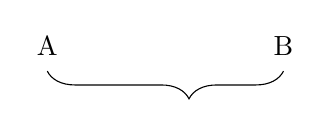
\begin{tikzpicture}
\draw(0,0)coordinate(A)node[above]{A} (3,0)coordinate(B)node[above]{B};
\coordinate(B) at (3,0);
\draw[decorate,decoration={brace,amplitude=10pt,aspect=0.6,mirror,raise=2pt}](A)--(B);
\end{tikzpicture}

$\wp=\ell+1 $

\begin{tikzpicture}
\fill[pattern=north east lines] (0,0) rectangle (2,1);
\end{tikzpicture}
\begin{tikzpicture}
\draw(0,0)node[ocirc]{}node[above]{a};
\draw(1,0)node[ocirc]{}node[above]{b};
\node[inner sep=0pt](a) at (0,0){};
\node[inner sep=5pt](b) at (1,0){};
\draw(a)--(b);
\end{tikzpicture}
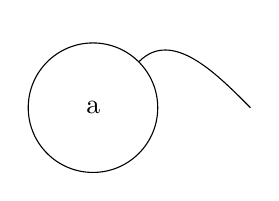
\begin{tikzpicture}
\draw(0,0) node[draw,circle,inner sep=0.5cm](a){a};
\draw(a) to [out=45,in=135]++(2,0);
\end{tikzpicture}
